%导言区
\documentclass[12pt]{ctexart}
\title{\vspace{-1.5cm} \zihao{3} \heiti \LaTeX 模板}
\date{}

%********************包的引用****************%
% 页面设置
\usepackage{fancyhdr}        % 页脚页眉
\usepackage{lastpage}        % 获取总共的页数
\usepackage{geometry}        % 设置页边距
% 修改摘要
\usepackage{abstract}
% 数学环境
\usepackage{amsmath}
\usepackage{amssymb}
% 矩阵斜省略号iddots
\usepackage{mathdots}
% 插入图片
\usepackage{graphicx} 		% 插入图片的宏包(can't graphics)
\usepackage{float} 			% 设置图片浮动位置的宏包
\graphicspath{{./figure/}}  % 搜索路径
\usepackage{subfigure} 		% 多图排版
% 三线表
\usepackage{booktabs}
% 间距宏包
\usepackage{setspace}
% 文字加颜色
\usepackage{color}
\usepackage{xcolor}
% 插入代码宏包
\usepackage{listings}
\usepackage{appendix} % 附录

%*******************全文格式设置********************%

% 设置纸张为A4,上下边距为3.2、2.8cm,左右边距为2.5cm 
\geometry{a4paper,left=2.5cm,right=2.5cm,top=2.5cm,bottom=2.5cm}

% 各级标题格式的设置
\setcounter{tocdepth}{4}     % 设置目录显示的深度为4
\setcounter{secnumdepth}{4}  % 设置章节显示的深度为4
\ctexset{
	% 黑体小三,居中对齐,段前段后30pt
	section={
		format=\zihao{-3} \heiti \centering,
		name = {,、},
		number = \chinese{section},
		aftername=\hspace{0pt},
		beforeskip=30pt,
		afterskip=30pt
	},
	subsection={
		format = \zihao{-3} \heiti \raggedright,
		beforeskip=18pt,
		afterskip=12pt
	},
	subsubsection={
		format=\fontsize{13pt}{20pt} \heiti \raggedright,
		beforeskip=12pt,
		afterskip=12pt,
	},
	paragraph={
		format=\zihao{-4} \songti \raggedright,
		beforeskip=6pt,
		afterskip=6pt,
	}
}

% 摘要格式设置
\setlength{\abstitleskip}{-1em} % 摘要标题和内容的间距
\setlength{\absleftindent}{6pt}
\setlength{\absrightindent}{6pt}
\renewcommand{\abstractnamefont}{\zihao{4} \centering \heiti}
\renewcommand{\abstracttextfont}{\zihao{-4} \songti}

% 附录格式设置
\lstset{
	numbers=left, % 行号显示在左边
	numberstyle=\tiny, % 行号字体为tiny
	basicstyle=\ttfamily, % 设置字体族
	breaklines=true, % 自动换行
	frame=shadowbox, % 边框
	% 设置关键词
	keywordstyle=\color{blue!70},
	morekeywords={}, % 设置更多的关键字,用逗号分隔
	% 设置注释样式(斜体)
	commentstyle=\itshape\color{red!50!green!50!blue!50},
	% 代码块边框颜色
	rulesepcolor=\color{red!20!green!20!blue!20},
	% 左右页边距
	xleftmargin=1em,xrightmargin=1em,
	% 上页边距
	aboveskip=-1em,
	% 背景颜色
	backgroundcolor=\color{white}
} 

% 设置页码
\pagestyle{fancy}     % 使用fancy风格
\fancyhf{}            % 清除所有的页眉页脚
\renewcommand\headrulewidth{0pt}   % 去除页眉横线
\fancyfoot[C]{\thepage}   % 页码

% 全文设置1.5倍间距
\setlength{\baselineskip}{20pt}     
% \renewcommand{\baselinestretch}{1.5}  % 全文设置1.5倍间距

% 参考文献样式
\bibliographystyle{plain}
% 定义参考文献的数字为右上角的命令:\supercite
% 1个参数,#1传参,\textsuperscript文本环境下的上标
\newcommand\supercite[1]{\textsuperscript{\cite{#1}}}


%******************正文区******************%
\begin{document}
\begin{spacing}{1.5}
	
\maketitle	% 设置标题
\setcounter{page}{1}  % 从此页开始编页码
% \thispagestyle{empty} % 不计此页页数
% \tableofcontents      % 显示目录

\vspace{-6.5em}
% \vspace*{-2.5cm} % 向上缩进
%**********************摘要*******************%
\begin{abstract}
	公交车是为市民出行提供服务的“准公共”产品。然后针对不同区域不同时间段的人流量情况,我们需要对公交车进行一定的调度,以使得在增加盈利的同时,兼顾“尽可能减少私家车使用以缓解城市交通拥堵”和“尽量让公众满意”两大目标。本文通过给出合理的“高峰”和“平峰”的定义,并在此基础上给出在转换期的最优化分布调度方案,最后在此基础上给出平峰和高峰的预测方法并对其进行验证。
	
	我们在具体环境(公交车成本为200,发车间隔为5min/辆,票价为:1元/人,载客量为84人/辆)下定义阈值为区分高峰和低峰的临界值:691;则相应高于阈值则为高峰,低于阈值则为低峰,通过定义阈值间接给出高峰和低峰的预测。利用排队论单目标混合模型,通过验证其在此环境下的阈值处的顾客损失率为0.0118,小于一进而证明在此定义的阈值处,刚好是高峰和低峰的分界处,则说明该定义合理。

	问题二环境与问题一相同,我们通过相应的改变发车频率进行分步调控,给出最终的调度方案(从高峰段到低峰段的调度时,选择5min间隔发车-->5/10min间隔交替发车-->10min间隔发车;在从低峰段到高峰段的调度时,则选择与之相反调度),使得盈利的大小均超过阈值。并将人流量作为研究指标,通过拟合调度前后各时间段盈利额与阈值的比较图,发现调度后每一个时间段的盈利额都在阈值界限上方,则说明此调度方案是合理的;通过将此调度方案放入不同人流量情况下,观察其每个时间段盈利额与阈值的比较图,若并非都在阈值上方,则说明此调度方案针对最开始所给数据是最优的。

	~\\
	\textbf{关键词:} \quad 排队论 \quad 调度模型\supercite{参考文献1}
\end{abstract}

\newpage % 新的一页

\section{问题重述}
	公交车是为市民出行提供服务的“准公共”产品。然后针对不同区域不同时间段的人流量情况,我们需要对公交车进行一定的调度,以使得在增加盈利的同时,兼顾“尽可能减少私家车使用以缓解城市交通拥堵”和“尽量让公众满意”两大目标。本文通过给出合理的“高峰”和“平峰”的定义,并在此基础上给出在转换期的最优化分布调度方案,最后在此基础上给出平峰和高峰的预测方法并对其进行验证\supercite{参考文献2}。
	
	公交车是为市民出行提供服务的“准公共”产品。然后针对不同区域不同时间段的人流量情况,我们需要对公交车进行一定的调度,以使得在增加盈利的同时,兼顾“尽可能减少私家车使用以缓解城市交通拥堵”和“尽量让公众满意”两大目标。本文通过给出合理的“高峰”和“平峰”的定义,并在此基础上给出在转换期的最优化分布调度方案,最后在此基础上给出平峰和高峰的预测方法并对其进行验证

\section{问题分析}
\subsection{问题一}
\begin{figure}[H]
	\centering
	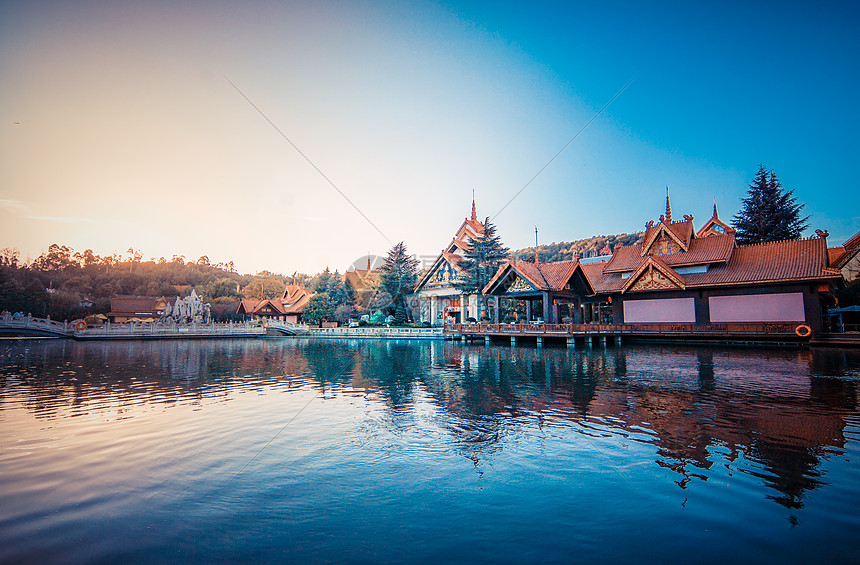
\includegraphics[width=0.4\textwidth]{风景.jpg}
	\caption{单图排版}
	\label{image1}
\end{figure}
\subsection{问题二}
	公交车是为市民出行提供服务的“准公共”产品。然后针对不同区域不同时间段的人流量情况,我们需要对公交车进行一定的调度,以使得在增加盈利的同时,兼顾“尽可能减少私家车使用以缓解城市交通拥堵”和“尽量让公众满意”两大目标。本文通过给出合理的“高峰”和“平峰”的定义,并在此基础上给出在转换期的最优化分布调度方案,最后在此基础上给出平峰和高峰的预测方法并对其进行验证。\supercite{参考文献3}
\subsection{问题三}
\subsection{问题四}

\section{模型的假设}

\section{符号说明}
\begin{center}
	\begin{tabular}{cc}
		\toprule[1.5pt]
		\makebox[0.3\textwidth][c]{符号}	&  \makebox[0.4\textwidth][c]{意义} \\
		\midrule[0.5pt]
		$ W $	    & 简单移动平均项 \\
		$ M_t $	    & 长期趋势项 \\
		\bottomrule[1.5pt]
	\end{tabular}
\end{center}

\section{模型建立、求解与检验}
\subsection{问题一}
\subsubsection{模型建立}
\subsubsection{模型求解}
\subsection{问题二}
\subsection{问题三}
\subsection{问题四}

\section{优缺点分析}
\subsection{优点}
\subsection{缺点}

% 参考文献
\bibliography{book} % 采用外面导入bib文件形式

\newpage

% 附录
\appendix
\ctexset{
	section={
		format=\zihao{-3} \heiti \centering,
		name = {附录,},
		number = \Alph{section},
		aftername=\hspace{12pt},
	}
}
\section{第1问源代码}
\begin{lstlisting}[title="OK.m",language=matlab]
% 代码段
clear,clc
disp('OK')
\end{lstlisting}

\section{第2问源代码}
{\color{red}{红色}}

\end{spacing}	
\end{document}